\setcounter{section}{0}

\section{Serie temporal}
Aunque existen series puramente aleatorias, el interés reside en aquellas formadas por la combinación de una componente aleatoria y una determinista. Con la modelización vamos a estudiar su comportamiento, estructura, patrones y correlaciones, entre otros, a fin de ser capaces de predecir el futuro gracias al pasado, es decir, la principal motivación para el estudio de las series temporales va a ser la predicción.

En ocasiones, para el correcto tratamiento de una serie temporal tenemos que trabajar bajo un supuesto muy importante: la estacionariedad. Intuitivamente, una serie es estrictamente estacionaria si el mecanismo que la genera no varía a lo largo del tiempo, asegurándonos así cierta estabilidad temporal. Más formalmente, se dice que un proceso es estrictamente estacionario si la función de distribución de un conjunto de sus $n$ variables aleatorias se mantiene idéntica para cualquier separación de tiempo $k$:
\begin{equation}
    F[Y_{t_{1}}, Y_{t_{2}},...,Y_{t_{n}}]=F[Y_{t_{1+k}}, Y_{t_{2+k}},...,Y_{t_{n+k}}] \quad \forall{t_{i}} \quad\textrm{con}\quad i = 1,...,n \quad\quad
    k \in Z
\end{equation}

Se puede apreciar que este supuesto es demasiado estricto ya que el mundo real no es completamente estático. En series temporales extraídas de datos reales, es muy complicado que el mecanismo generador se mantenga idéntico con el paso del tiempo, por lo que realmente se trabaja con una estacionariedad débil o en covarianza, definida por las siguientes características:
\begin{equation}
    E[Y_{t}]=\mu<\infty \quad \quad \forall{t}
\end{equation}
\begin{equation}
    Var(Y_{t})=\sigma^2<\infty \quad \quad \forall{t}
\end{equation}
\begin{equation}
    Cov(Y_{t},Y_{t+k})=E[(Y_{t}-\mu)(Y_{t+k}-\mu)]<\infty \quad \quad \forall{t}
\end{equation}

Sabiendo esto, podemos apreciar que un proceso estacionario siempre está bajo control en el sentido de que las variables aleatorias van a evolucionar entorno a una media y varianza finitas, además la covarianza entre dos observaciones dependerá únicamente del rezago temporal $k$ que las separa (Cuando hablemos en este trabajo de estacionariedad nos referiremos siempre a la débil) \cite{shumway2010time}.

Para poder estudiar las dependencias temporales de este tipo de datos conviene conocer ciertas funciones. La primera de ellas es la función de autocovarianzas de una serie estacionaria, que mide la dependencia lineal entre dos puntos de la serie separados por un espacio de tiempo $k$. La autocovarianza para el rezago $k$ se define de la siguiente manera:
\begin{equation}
    \gamma_{k}=Cov(Y_{t},Y_{t+k})=E[(Y_{t}-\mu)(Y_{t+k}-\mu)] \quad \quad k \in N
\end{equation}

La autocovarianza depende de las unidades de medida de la variable, por lo que generalmente se suele usar la función de autocorrelación (FAC o ACF) en la que trabajamos de la misma manera pero utilizando la correlación entre pares de variables separadas por un rezago $k$:
\begin{equation}
    \rho_{k}=\frac{\gamma_{k}}{\gamma_{0}}
\end{equation}

Se puede demostrar que $-1 \leq \rho_{k} \leq 1$ para todo $k$, pudiéndose así evaluar el grado de autocorrelación de una serie de acuerdo a estos extremos. Bajo estacionariedad, la autocorrelación entre variables va desapareciendo, se va desvaneciendo, es por esto que bajo estacionariedad cuando $k\rightarrow \infty$ se tiene que $\rho_{k}\rightarrow 0$ \cite{gujarati}.

Conviene también mencionar la función de autocorrelación parcial (FACP o PACF). Esta función trabaja de manera similar a la de autocorrelación solo que no tiene en cuenta la dependencia lineal provocada por las variables intermedias $Y_{t+1}, Y_{t+2},...,Y_{t+k-1}$.

Existen varios enfoques orientados al análisis de series temporales, aunque quizás merezca la pena destacar dos:

\begin{itemize*}
  \item[$\bullet$] \textbf{Enfoque determinista}: Se busca expresar la serie temporal como la combinación de varias componentes. Cada una de las componentes recoge cierta información de la serie (estacionalidad, tendencia, ciclo e irregular). La combinación de estas componentes dependerá de la evolución de la serie (aditiva o multiplicativa). Técnicas muy utilizadas propias de este enfoque son las de suavizado, que buscan realizar inferencias hacia el futuro de forma sencilla.
  \item[$\bullet$] \textbf{Metodología Box-Jenkins}: Este tipo de modelado busca ajustar el mejor modelo a nuestros datos entre varios posibles, para ello se comparan algunas características de la serie con las propias de los distintos modelos. Una vez elegido el modelo a ajustar se estiman los parámetros y se realiza una validación para confirmar que el modelo elegido es el óptimo. Esta familia de modelos se apoyan en valores pasados de la serie para realizar inferencias por lo que se necesita el cumplimiento de algunos supuestos estadísticos básicos.
\end{itemize*}


%%%%%%%%%%%%%%%%%%%%%%%%%%%%%%%%%%%%%%%%%%%%%%%%%%%%%%%%%%%%%%%%%%%%%%%%%%%%%%%%%%%%%%%%%%%%%%%%%%%%%%%%%%%%%%%%%%%%%%%%%%%%%%%%%%%%%%%%%%%%%%%%
%%%%%%%%%%%%%%%%%%%%%%%%%%%%%%%%%%%%%%%%%%%%%%%%%%%%%%%%%%%%%%%%%%%%%%%%%%%%%%%%%%%%%%%%%%%%%%%%%%%%%%%%%%%%%%%%%%%%%%%%%%%%%%%%%%%%%%%%%%%%%%%%


\section{Enfoque determinista}

Este tipo de enfoque es bastante común ya que permite obtener una visión general y rápida de la evolución de cualquier serie temporal, pudiéndose incluso obtener inferencias del futuro cercano de no mala calidad. Además, la interpretación de los resultados es bastante intuitiva.

En este caso la serie temporal se expresa como el resultado de la suma de una función de $t$ más un error aleatorio que se supone ruido blanco:
\begin{equation}
    Y_{t} = f(t) + a_t \quad \text{con} \quad a_t \approx RB(0, \sigma^2)
\end{equation}

Lo que se busca es aproximar $f(t)$ a fin de conocer cómo funciona la correspondiente serie temporal. Para ello se busca descomponer la serie en varias componentes, cada una de las cuales almacena cierta información de la serie estudiada.  Las principales componentes son:

\begin{itemize*}
  \item[$\bullet$] \textbf{Tendencia} ($T_t$): Muestra la evolución de la serie temporal a largo plazo. Nos ayuda a conocer hacia dónde se dirige la serie de forma general, es decir, en media.
  \item[$\bullet$] \textbf{Estacionalidad} ($S_t$): Se refiere a variaciones que ocurren siguiendo un patrón basado en periodos temporales cortos y conocidos (crecimiento en verano y disminución en invierno, patrones trimestrales, etc…)
  \item[$\bullet$] \textbf{Ciclo} ($C_t$): Variaciones similares a las de la estacionalidad pero que siguen periodos muchos más largos (generalmente superiores al año). Esta componente es típica de series económicas y en muchos casos es difícil de estimar.
  \item[$\bullet$] \textbf{Fluctuaciones irregulares} ($a_t$): Recoge las fluctuaciones de la serie que no siguen una pauta periódica ni tendencia reconocible, razón por la cual a esta componente también se le llama ``ruido".
\end{itemize*}

En un modelo determinado, no tienen por qué estar presentes las cuatro componentes, en algunos casos puede que algunas de ellas no haga presencia en la serie estudiada. Además se supone que la serie puede ser expresada como la suma o producto de sus componentes, lo que da origen a dos modelos:

\begin{itemize*}
  \item[$\bullet$] \textbf{Modelo aditivo}: Propio de las series temporales que conservan una amplitud constante a lo largo del tiempo. Supone que las observaciones son el resultado de la suma de sus componentes.
      \begin{equation}
        Y_t = T_t + S_t + C_t + a_t
      \end{equation}
  \item[$\bullet$] \textbf{Modelo multiplicativo}: Este modelo se suele ajustar a aquellas series con una amplitud dependiente del tiempo. Supone que las observaciones se generan de la multiplicación de sus componentes.
      \begin{equation}
        Y_t = T_t \times S_t \times C_t \times a_t
      \end{equation}
\end{itemize*}

\begin{figure}
\begin{subfigure}{.5\textwidth}
  \centering
  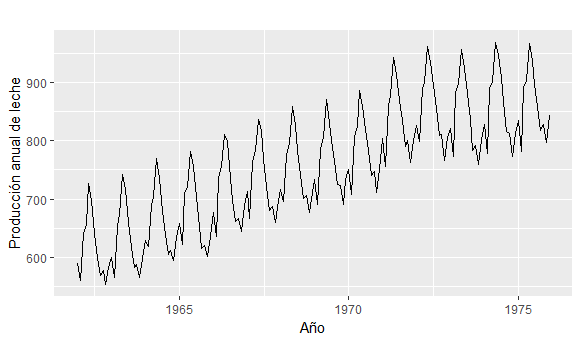
\includegraphics[width=.8\linewidth]{Images/Conceptos/leche.png}
  \caption{Estructura aditiva}
  \label{fig:sfig1}
\end{subfigure}
\begin{subfigure}{.5\textwidth}
  \centering
  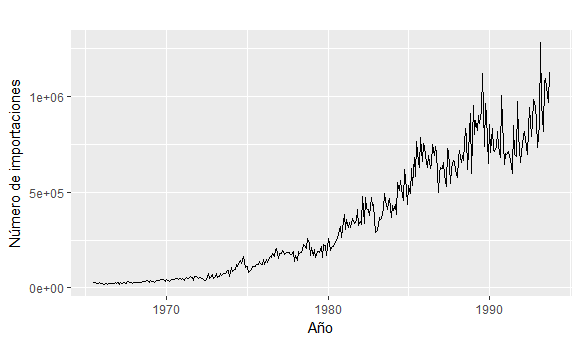
\includegraphics[width=.8\linewidth]{Images/Conceptos/importaciones.png}
  \caption{Estructura multiplicativa}
  \label{fig:sfig2}
\end{subfigure}
\caption{Comparación entre un modelo aditivo y multiplicativo}
\label{ad_mult}
\end{figure}

En la Figura \ref{ad_mult} se muestran ejemplos de ambos modelos. Identificar y entender el mecanismo que genera la serie temporal nos permitirá realizar predicciones fiables, además de ser capaces de entender mejor el proceso que genera los datos. Esto lo vamos a conseguir con la descomposición de la serie en subseries de acuerdo a las distintas componentes. Gracias a esta descomposición vamos a poder estudiar la evolución individual de cada componente, lo que nos permitirá identificar posibles patrones a fin de reproducir el comportamiento de la serie.

\subsection{Estimación de la tendencia}

Normalmente la tendencia es una de las componentes que más interesa estimar, ya que mediante técnicas sencillas podemos conocer la evolución a largo plazo de la serie. Existen varias técnicas para la extracción de la tendencia, el uso de unas u otras dependerá de la estructura y de la extensión de la serie que estemos estudiando.

En ocasiones la tendencia sigue un comportamiento fácilmente modelizable por una función $h(t)$ dependiente del tiempo $t$. La estimación de $h(t)$ se suele realizar por el método de los mínimos cuadrados. La estimación de los parámetros no va a suponer ningún problema gracias a la potencia computacional disponible hoy en día pero si lo supondrá la elección del modelo.

Algunas veces es sencillo identificar visualmente la función a usar para aproximar la tendencia ya que esta puede mostrar una evolución muy marcada (lineal, exponencial…). En caso contrario se puede probar a ajustar distintas funciones a fin de ver cuál de ellas se ajusta mejor. La elección de la función óptima se basa en indicadores estadísticos como el $R^2$ o la significatividad de los parámetros, aunque muchas veces basta con observar la serie temporal para decidirse por una u otra.

Algunas de las funciones más utilizadas para la estimación de la tendencia son:
\begin{description}
  \item[$\bullet$ Función lineal:]
      \begin{equation}
        h(t) = \alpha_0 + \alpha_1 t \quad con \quad \alpha_0, \alpha_1 \in \mathbb{R}
      \end{equation}
  \item[$\bullet$ Función cuadrática:]
      \begin{equation}
        h(t) = \alpha_0 + \alpha_1 t + \alpha_2 t^2 \quad con \quad \alpha_0, \alpha_1, \alpha_2 \in \mathbb{R}
      \end{equation}
  \item[$\bullet$ Función exponencial:]
      \begin{equation}
        h(t) = e^{\alpha_0 + \alpha_1 t} \quad con \quad \alpha_0, \alpha_1 \in \mathbb{R}
      \end{equation}
  \item[$\bullet$ Función logística:]
      \begin{equation}
        h(t) = \frac{e^{\alpha_0 + \alpha_1 t}}{1 + e^{\alpha_0 + \alpha_1 t}} \quad con \quad \alpha_0, \alpha_1 \in \mathbb{R}
      \end{equation}
\end{description}

En algunas ocasiones la serie temporal a estudiar no muestra un mismo comportamiento continuo a largo plazo por lo que ajustar este tipo de funciones supondría una gran pérdida de información. En este caso nos sería de gran utilidad ajustar un modelo que tuviese en cuenta intervalos más cortos de tiempo, facilitándonos así la visualización de la tendencia. El método de la media móvil se ajusta a esta problemática.

\subsubsection{Método de la media móvil}

Este método nos permite obtener una visualización rápida de la tendencia de la serie ya que trabaja con medias. Lo que hace es calcular medias de acuerdo a intervalos de longitud $p$, estos intervalos se van actualizando, eliminando la primera observación y añadiendo una nueva. Para calcular una media de orden $p$ sobre la serie $Y_t$ se recurre a lo siguiente:
\begin{equation}
    Y'_{t} = \frac{1}{p}\left(Y_{t-\left(\frac{p-1}{2}\right)}+...+Y_{t-1}+Y_t+Y_{t+1}+...+Y_{t+\left(\frac{p-1}{2}\right)}\right)
\end{equation}

Este método consigue eliminar el ruido y las fluctuaciones mediante los promedios, dejando a la vista la tendencia de la serie. En ocasiones hay que fijar $p$ de acuerdo a la estructura temporal de la serie para evitar extraer conclusiones erróneas sobre la tendencia.  Debido a la propia naturaleza del método incurrimos en una pérdida de $p$ observaciones.

\subsection{Estimación del ciclo}
La componente correspondiente al ciclo suele ser la más difícil de detectar y estimar, ya que aunque presenta variaciones más o menos recurrentes en el tiempo suelen ser resultado de la combinación de efectos muy variados con periodos diferentes. Debido a que muchas veces no es posible separar la tendencia del ciclo, estas dos componentes se estiman conjuntamente mediante las técnicas aplicadas a la estimación de la tendencia.

\subsection{Estimación de la estacionalidad}
Al igual que con la tendencia, existen varias aproximaciones a la hora de estimar la componente estacional. Debido a su naturaleza ondulatoria en ocasiones es posible aproximar esta componente a través de una función $g(t)$ periódica de periodo $s$:
\begin{equation}
    g(t) = g(t + s) = g(t + 2s)
\end{equation}

El periodo $s$ se corresponde al patrón de estacionalidad de la serie ($s = 4$ para datos trimestrales, $s = 12$ para datos mensuales…). Este tipo de funciones suelen estar formadas por una combinación de funciones armónicas. Estas técnicas suelen ajustarse  correctamente a estacionalidades con fluctuaciones complejas.

Otra forma de aproximar $g(t)$ es mediante variables \textit{dummy}. Estas variables recogen las variaciones debidas a la periodicidad estacional, de esta forma podemos expresar $g(t)$ como:
\begin{equation}
    g(t) = \sum_{i=1}^{S}(\lambda_{i} d_{it})
\end{equation}

\noindent donde $d_{it}$ son variables \textit{dummys} que toman el valor $1$ si el dato pertenece a ese periodo estacional y $0$ en caso contrario. El coeficiente $\lambda_{i}$ indica la variación correspondiente al periodo estacional $i$. Para estimar este factor estacional, si la estacionalidad es estable en el tiempo, basta con realizar la media de las observaciones correspondientes a cada periodo, en caso contrario no conviene resumir las distintas medias de cada periodo en un solo factor por que no describirá correctamente el comportamiento variable de la estacionalidad. En este último caso convendría ajustar alguna función matemática más compleja a esta componente.

\subsection{Estimación de la componente irregular}
El análisis de los residuos nos puede ser de gran utilidad a la hora de ver si hemos conseguido extraer correctamente todas las componentes. Sin los residuos (o componente irregular) no parecen mostrar ningún patrón, significa que hemos sido capaces de extraer todas las causas deterministas que componían la serie. Es posible obtener la componente irregular de la siguiente manera:
\begin{equation}
    Y_t - Y'_t - S_t = a_t
\end{equation}
\begin{equation}
    \frac{Y_t}{Y'_t \times S_t} = a_t
\end{equation}

En la Figura \ref{decomp} se muestra un ejemplo de descomposición de una serie temporal.
\begin{figure} [t]
\begin{subfigure}{.5\textwidth}
  \centering
  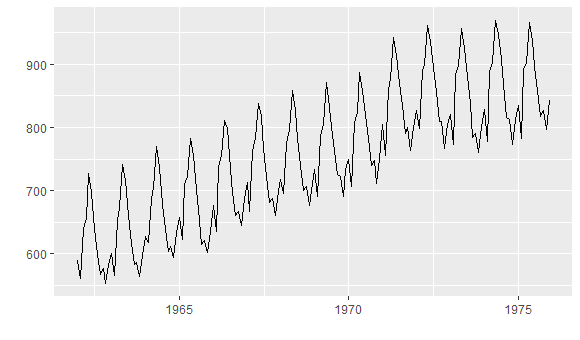
\includegraphics[width=.8\linewidth]{Images/Conceptos/serie.png}
  \caption{Serie original}
  \label{fig:sfig1}
\end{subfigure}
\begin{subfigure}{.5\textwidth}
  \centering
  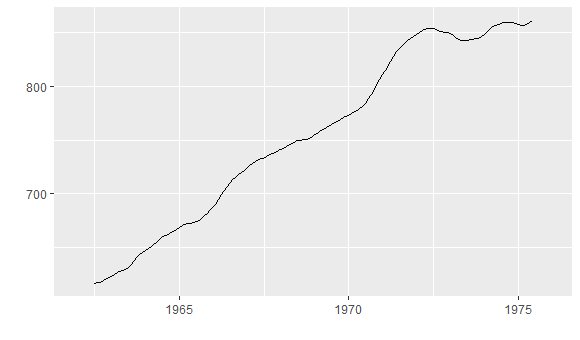
\includegraphics[width=.8\linewidth]{Images/Conceptos/tend.png}
  \caption{Tendencia}
  \label{fig:sfig2}
\end{subfigure}
\begin{subfigure}{.5\textwidth}
  \centering
  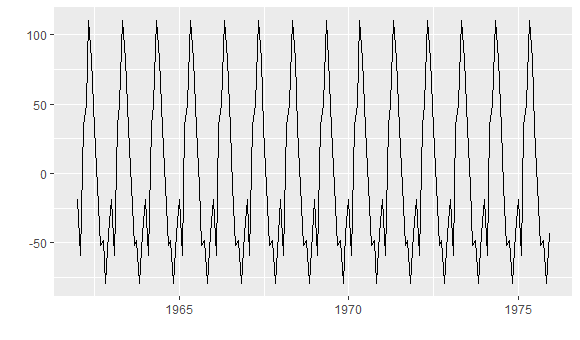
\includegraphics[width=.8\linewidth]{Images/Conceptos/season.png}
  \caption{Estacionalidad}
  \label{fig:sfig1}
\end{subfigure}
\begin{subfigure}{.5\textwidth}
  \centering
  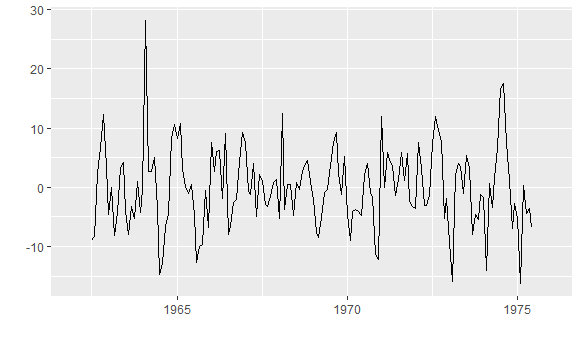
\includegraphics[width=.8\linewidth]{Images/Conceptos/random.png}
  \caption{Irregular}
  \label{fig:sfig2}
\end{subfigure}
\caption{Descomposición de la serie correspondiente a la producción de leche anual (Fuente:~\protect\citeNP{datamarket})}
\label{decomp}
\end{figure}


\subsection{Técnicas de suavizado}

Este tipo de técnicas nos permiten reducir o eliminar la aleatoriedad de la serie temporal permitiendo así una observación más nítida de sus componentes. Además nos ayudan a  predecir a corto plazo sin la necesidad de recurrir a modelos matemáticos complejos. Aunque este tipo de técnicas se pueden usar para cualquier tipo de serie temporal, suelen aplicarse más a aquellas que presentan una estructura inestable, con unas componentes menos marcadas o inexistentes debido a su naturaleza adaptativa a nivel local.

Uno de los suavizados más aplicados debido a su sencillez es el de medias móviles, ya explicado en apartados anteriores. Otros suavizados más complejos como el de \textit{splines} o \textit{kernel} (Anexo I) ofrecen también muy buenos resultados, aunque obviamente son mucho más costosos computacionalmente.

\subsubsection{Suavizado exponencial}
El suavizado exponencial es una media móvil ponderada en la que los valores más cercanos en el tiempo se ponderan más que los más alejados, a diferencia del suavizado de media móvil donde todos los valores influyen de igual manera.

El cálculo de la serie alisada se realiza de la siguiente manera:
\begin{equation}
   Y'_{t} = \alpha Y_{t} + (1 - \alpha)\thinspace Y_{t-1} + (1 - \alpha)^2 \thinspace Y_{t-2} + ... = \alpha \sum_{i=0}^{\infty} (1 - \alpha)^i \thinspace Y_{t-i} \quad \text{con} \quad 0 < \alpha < 1
\end{equation}

Como se puede apreciar, la serie alisada en el tiempo $t$ es resultado de la suma ponderada de todos los valores anteriores. Esta ponderación supone que los valores más recientes tienen una mayor influencia y esta influencia se va dispersando con el tiempo. Al parámetro $\alpha$ se le conoce como el factor de suavización y de él depende la importancia que se le da a los valores pasados y recientes. Este factor suele ser fijado por el investigador y dependerá principalmente de la estructura y evolución de la serie.

Se puede apreciar que para calcular cada nuevo valor alisado de la serie es necesario realizar los cálculos sobre todos los valores anteriores.  Para solventar este problema se suele recurrir a una expresión resultado de la aplicación de transformaciones matemáticas a la expresión (19) que da como resultado las siguientes fórmulas correspondientes al valor alisado y a la predicción de la serie, respectivamente:
\begin{equation}
   Y'_{t} = \alpha Y_{t} + (1 - \alpha)\thinspace Y'_{t-1}
\end{equation}
\begin{equation}
   \widehat{Y}_{t+1} = \alpha Y_{t} + (1 - \alpha)\thinspace \widehat{Y}_{t}
\end{equation}

Sabiendo esto podemos apreciar que:
\begin{equation}
   Y'_{2} = \alpha Y_{2} + (1 - \alpha)\thinspace Y'_{1}
\end{equation}

Por lo que el valor asignado a $Y'_{1}$ va a jugar un papel fundamental en el alisado de la serie. Existen varias posibilidades a elegir para fijar este valor (que sea igual a $Y_{1}$ o utilizar la media de la serie son algunas de ellas) que dependerán de la estructura y características propias de la serie.

Sabiendo esto, podemos apreciar mejor la importancia del factor de suavizado. Un $\alpha$ cercano a 0 significa que la parte alisada se tendrá más en cuenta y esto como consecuencia generará una suavización sin fluctuaciones. Un $\alpha$ cercano a 1 dará más peso a los valores más recientes de la serie generando así una suavización que tiene más en cuenta las fluctuaciones.

El suavizado aquí explicado es el simple y sirve de base para otros más complejos con una estructura también exponencial, capaces de adaptarse a tendencia y patrones estacionales mucho más complicados. En la Figura \ref{suav} se muestra un ejemplo de aplicación de estos suavizados.
\begin{figure} [t]
\begin{subfigure}{.5\textwidth}
  \centering
  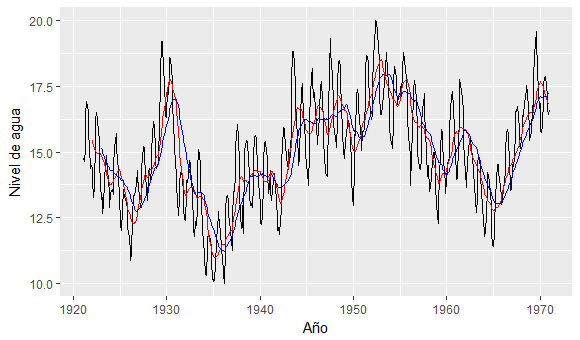
\includegraphics[width=.8\linewidth]{Images/Conceptos/ma.png}
  \caption{Medias móviles}
  \label{fig:sfig1}
\end{subfigure}
\begin{subfigure}{.5\textwidth}
  \centering
  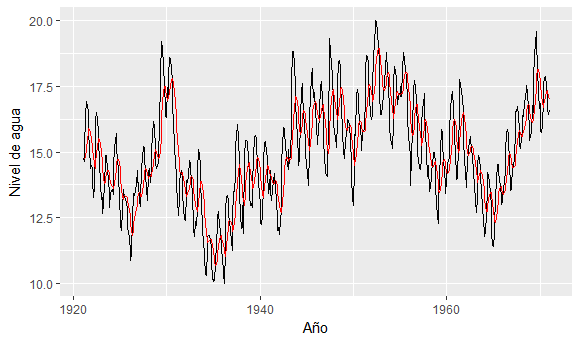
\includegraphics[width=.8\linewidth]{Images/Conceptos/exp.png}
  \caption{Exponencial simple}
  \label{fig:sfig2}
\end{subfigure}
\begin{subfigure}{.5\textwidth}
  \centering
  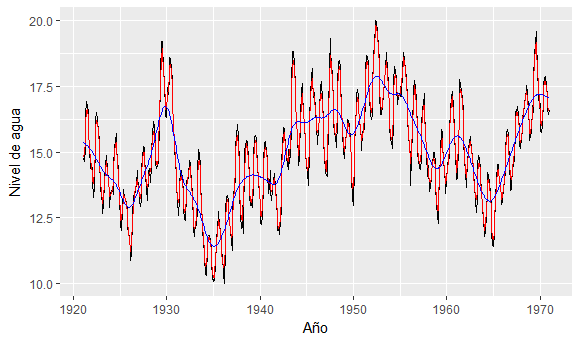
\includegraphics[width=.8\linewidth]{Images/Conceptos/ker.png}
  \caption{Kernel}
  \label{fig:sfig1}
\end{subfigure}
\begin{subfigure}{.5\textwidth}
  \centering
  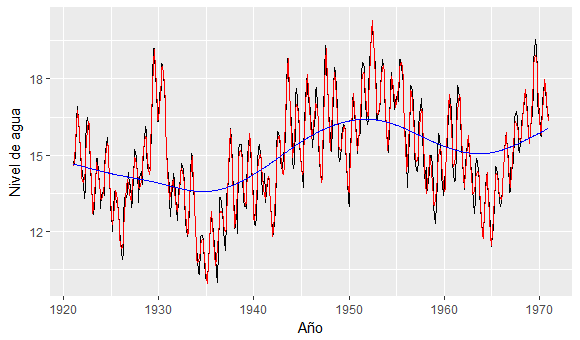
\includegraphics[width=.8\linewidth]{Images/Conceptos/spln.png}
  \caption{Spline}
  \label{fig:sfig2}
\end{subfigure}
\caption{Suavizado de la serie correspondiente al nivel mensual de agua del lago Erie (Fuente:~\protect\citeNP{datamarket})}
\label{suav}
\end{figure}


%%%%%%%%%%%%%%%%%%%%%%%%%%%%%%%%%%%%%%%%%%%%%%%%%%%%%%%%%%%%%%%%%%%%%%%%%%%%%%%%%%%%%%%%%%%%%%%%%%%%%%%%%%%%%%%%%%%%%%%%%%%%%%%%%%%%%%%%%%%%%%%%
%%%%%%%%%%%%%%%%%%%%%%%%%%%%%%%%%%%%%%%%%%%%%%%%%%%%%%%%%%%%%%%%%%%%%%%%%%%%%%%%%%%%%%%%%%%%%%%%%%%%%%%%%%%%%%%%%%%%%%%%%%%%%%%%%%%%%%%%%%%%%%%%


\section{Metodología Box-Jenkins}
La metodología Box-Jenkins fue desarrollada por George E. P. Box y Gwilym Jenkins en 1976 y se sustenta en los modelos ARIMA \cite{BoxJenkins2008}. Supone que la serie temporal es una realización de un proceso estocástico determinado y modelizable. Esta metodología busca encontrar un modelo que se ajuste a los datos y que nos permita realizar predicciones fiables a corto y medio plazo.

\subsection{Modelos ARIMA}
Para comprender este modelo vamos a realizar un pequeño recorrido por los distintos modelos que le componen.

\subsubsection{Procesos autorregresivos}
Algunas series temporales están muy influenciadas por sus valores pasados, en estos casos se ajusta un tipo de modelo autorregresivo en el que el valor presente de la variable depende de los valores pasados más una pequeña innovación contemporánea (parte aleatoria). Este modelo se conoce como autorregresivo y se suele denotar por las siglas AR. Si la variable se ve influenciada por sus valores pasados hasta el retardo $t-p$ hablamos de un modelo autorregresivo de orden $p$ o AR($p$). Sabiendo esto, podemos definir el modelo de la siguiente manera:
\begin{equation}
    Y_{t}=\phi_{1} Y_{t-1} + \phi_{2} Y_{t-2} + \phi_{3} Y_{t-3}+...+\phi_{p} Y_{t-p}+a_{t}
\end{equation}

\noindent con $\phi_i$ parámetros a estimar y $a_{t}$ ruido blanco.

Para estudiar la estacionariedad vamos a expresar el modelo mediante su operador de retardos:
\begin{equation}
    (1-\phi_{1}L-\phi_{2}L^{2}-...-\phi_{p}L^{p})Y_{t} = a_{t}
\end{equation}

\begin{equation}
    \phi_{p}(L)Y_{t} = a_{t}
\end{equation}

\noindent donde $\phi_{p}(L)$ se conoce como polinomio autorregresivo, siendo $(\phi_{1};\phi_{2};...;\phi_{p})$ su vector de parámetros. Este polinomio va a tener generalmente $p$ raíces diferentes por lo que se puede expresar como:
\begin{equation}
    \phi_{p} = \prod_{i=1}^{p}(1-L_{i}^{-1}L)
\end{equation}

Está demostrado que este proceso será estacionario si y solo si el módulo de las raíces de su polinomio autorregresivo está fuera del círculo unidad:
\begin{equation}
    \mid L_{i}^{-1}\mid < 1 \quad \forall{i}
\end{equation}

Además para poder garantizar completamente la estacionariedad de un proceso autorregresivo, éste debe depender  únicamente de su pasado y no de su futuro, lo cual se cumple en la mayor parte de series temporales y además debe ser invertible, es decir, debe cumplirse que:
\begin{equation}
    \sum_{i=1}^{p} \phi_{i}^{2} < \infty
\end{equation}

La función de autocorrelación se caracteriza por aproximarse a cero conforme $k \rightarrow \infty$, pudiendo ser este decrecimiento oscilante.

\subsubsection{Procesos de medias móviles}
En ocasiones se dan casos en los que para una serie temporal determinada, un modelo en el que el valor actual depende de las innovaciones contemporáneas y pasadas hasta el retardo $t-q$ se ajusta correctamente. Los modelos sustentados en estos principios se conocen como modelos de medias móviles de orden $q$ o MA($q$), se definen de la siguiente forma:
\begin{equation}
    Y_{t} =  a_{t}-\theta_{1}a_{t-1}-\theta_{2}a_{t-2}-...-\theta_{q}a_{t-q}
\end{equation}

\noindent con $\theta_i$ parámetros a estimar y $a_{t-i}$ ruido blanco.

Si procedemos como antes, tenemos que este proceso se puede representar mediante el operador de retardos:
\begin{equation}
    Y_{t} = \theta_{q}(L)a_{t}
\end{equation}

\noindent donde el polinomio de medias móviles se puede expresar a través de sus $q$ raíces:
\begin{equation}
    \theta_{q}(L) =  \prod_{i=1}^{q}(1-L_{i}^{-1}L)
\end{equation}

No es necesario imponer ninguna restricción sobre los parámetros $\theta_{1}, \theta_{2},...,\theta_{q}$ para garantizar la estacionariedad, sin embargo se necesita que el módulo de las raíces del polinomio de medias móviles esté fuera del círculo unidad para garantizar la invertibilidad:
\begin{equation}
\mid L_{i}^{-1}\mid < 1 \quad \forall{i}
\end{equation}

En este caso la función de autocorrelación se caracteriza por sufrir un corte abrupto a partir del retardo $q$.

\subsubsection{Procesos autorregresivos de medias móviles}
Este modelo determina el valor de $Y_{t}$ a partir de su pasado hasta el retardo $p$, de su innovación contemporánea y de las pasadas hasta el retado $q$. Se denota como ARMA($p$,$q$) y su expresión es la siguiente:
\begin{equation}
    Y_{t} = a_{t} + \sum_{i=1}^{p} \phi_{i} Y_{t-i} + \sum_{i=1}^{q} (-\theta_{i}) a_{t-i}
\end{equation}

Al tratar con ambos procesos a la vez en términos del operador de retardos tenemos lo siguiente:
\begin{equation}
    \phi_{p}(L)Y_{t} = \theta_{q}(L)a_{t}
\end{equation}

La estacionariedad del proceso dependerá de las condiciones de la parte autorregresiva, es decir, será estacionario siempre que el módulo de las raíces del polinomio autorregresivo esté fuera del círculo unidad, y la invertibilidad de la parte de medias móviles, o lo que es lo mismo, el módulo de las raíces del polinomio de medias móviles debe estar fuera del círculo unidad.

La función de autocovarianzas se caracteriza por ser infinita y la de autocorrelación por decrecer rápidamente hacia cero a medida que aumenta $k$.

\subsubsection{Procesos autorregresivos integrados de medias móviles}
Hemos visto que un proceso ARMA es estacionario si su parte autorregresiva lo es. La no estacionariedad del modelo se puede presentar entonces de dos formas distintas:
\begin{equation}
\mid L_{i}^{-1}\mid > 1 \quad \forall{i}
\end{equation}
\begin{equation}
\mid L_{i}^{-1}\mid = 1 \quad \forall{i}
\end{equation}

\noindent siendo $L_{i}$ las raíces del polinomio autorregresivo. En economía, que es dónde usualmente se utilizan este tipo de modelos, lo común es encontrarse con el segundo caso (raíz unitaria) en el que cual la serie se comporta más o menos igual a lo largo del tiempo variando únicamente de nivel. Para solucionar esto se recurren a los modelos autorregresivos integrados de medias móviles o ARIMA. Para ver cómo funcionan comencemos factorizando la parte autorregresiva del modelo general:
\begin{equation}
\phi_{p}(L)Y_{t} = (1-L_{1}^{-1}L)\cdot(1-L_{2}^{-1}L)\cdot...\cdot(1-L_{p}^{-1}L)
\end{equation}

Supongamos que tenemos $d$ raíces unitarias en esta parte autorregresiva, en ese caso podremos agrupar de la siguiente forma:
\begin{equation}
\phi_{p}(L)Y_{t} = \gamma_{p-d}(L)\cdot(1-L)^{d}
\end{equation}

Hemos agrupado las $d$ raíces unitarias en el término $(1-L)^{d}$ por lo que si ahora sustituimos en el modelo general tenemos que:
\begin{equation}
\gamma_{p-d}(L)\cdot(1-L)^{d}\cdot Y_{t}=\theta_{q}(L)a_{t}
\end{equation}
\begin{equation}
\gamma_{p-d}(L)\cdot\Delta^{d}Y_{t}=\theta_{q}(L)a_{t}
\end{equation}

Aquí $\gamma_{p-d}(L)$ es estacionario ya que no incluye a las raíces unitarias dado que las hemos conseguido eliminar diferenciando $Y_{t}$ $d$ veces. Por lo tanto ahora tenemos que el proceso que define a $\Delta^{d}Y_{t}$ es estacionario. Conociendo esto podemos afirmar que un modelo ARIMA no es más que un modelo ARMA diferenciado $d$ veces por lo que está compuesto de los parámetros $p$, $d$ y $q$, ARIMA($p, d, q$).

Como se puede apreciar el modelo ARIMA aúna las principales características de otros modelos. El objetivo de la metodología Box-Jenkins va a ser elegir los valores óptimos de los parámetros que definen al ARIMA para asegurarnos un ajuste óptimo de nuestros datos.

\subsection{Etapas}
En un principio la metodología Box-Jenkins estaba compuesta por tres etapas pero con el paso del tiempo han sido varios los autores que han defendido añadir alguna más \cite{etapas}. Nosotros consideraremos las siguientes etapas:
\begin{itemize*}
    \item[$\bullet$]Preparación de los datos
    \item[$\bullet$]Identificación y selección del modelo
    \item[$\bullet$]Estimación de los parámetros
    \item[$\bullet$]Validación del modelo
    \item[$\bullet$]Predicción
\end{itemize*}

\subsubsection{Preparación de los datos}
Como ya hemos visto, para que una serie sea estacionaria es necesario que no tenga tendencia y que la varianza sea constante. En la mayor parte de casos es posible observar esto mediante el estudio gráfico de los datos. Si nuestra serie muestra una evolución a largo plazo con pendiente, o la varianza parece evolucionar en el tiempo, es posible que nos encontremos ante una caso de no estacionariedad y necesitaremos tratar nuestra serie a fin de poder aplicar esta metodología.

En otras ocasiones, bien porque la gráfica no nos aporta mucha información o bien porque queremos asegurarnos estadísticamente de la estacionariedad de la serie, se recurre a distintos test estadísticos capaces de contrastar la estacionariedad de la serie estudiada. Uno de los más conocidos es la prueba de la raíz unitaria de Dickey Fuller.

En el caso de trabajar bajo no estacionariedad en tendencia se recomienda diferenciar la serie hasta conseguir eliminarla. Es aquí donde se define el valor del parámetro $d$ del ARIMA.

Si estamos tratando con una serie no estacionaria en varianza se suele recomendar aplicar alguna transformación a los datos que estabilice la varianza. Suele funcionar muy bien aplicar logaritmos a la serie aunque en ocasiones también se suele aplicar la transformación Box-Cox ya que además consigue aproximar la distribución de $Y_t$ a una normal:
\begin{equation}
Z(\lambda) =
\begin{cases}
\frac{y^\lambda - 1}{\lambda} & \text{si } \lambda \neq 0 \\
\log(y) & \text{si } \lambda = 0
\end{cases}
\end{equation}

\subsubsection{Identificación y selección del modelo}
Una vez preparada la serie debemos identificar el modelo a ajustar. En esta fase lo que principalmente se busca es elegir los valores óptimos de $p$ y $q$. Observando la FAC y FACP podemos estudiar la evolución de la autocorrelación de la serie, pudiendo así identificarla con alguna estructura típica de los distintos modelos estudiados.

En apartado anteriores hemos visto que por definición la FAC de un proceso autorregresivo se aproxima a cero conforme $k \rightarrow \infty$ y que la FAC de un proceso de medias móviles sufre un corte abrupto a partir del retardo $q$. A partir de este tipo de características es posible construir la Tabla \ref{identificacion}. Este tipo de tablas nos aportan información valiosa para una selección óptima del modelo.

\begin{table}[]
\centering
\label{my-label}
\begin{tabular}{|l|c|c|}
\hline
\multicolumn{1}{|c|}{} & FAC                            & FACP                           \\ \hline
AR($p$)                  & Decrece sin anularse           & Se anula para $j \textgreater p$ \\ \hline
MA($q$)                  & Se anula para $j \textgreater q$ & Decrece sin anularse           \\ \hline
ARMA($p,q$)              & Decrece sin anularse           & Decrece sin anularse           \\ \hline
\end{tabular}
\caption{Identificación de los distintos modelos}
\label{identificacion}
\end{table}

En la Figura \ref{comp_acf_pacf} se muestran las FAC teóricas para algunos modelos. Este tipo de identificación tiene un pequeño componente subjetivo debido a la propia interpretación de los correlogramas por lo que la experiencia del investigador juega un papel fundamental en la selección del modelo.

\begin{figure} [t]
\begin{subfigure}{.5\textwidth}
  \centering
  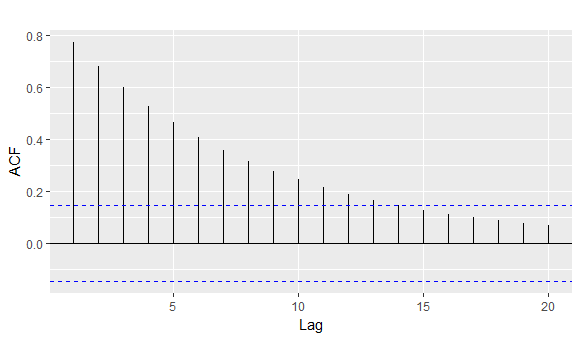
\includegraphics[width=.8\linewidth]{Images/Conceptos/ar_teorico.png}
  \caption{FAC de un proceso autorregresivo}
  \label{fig:sfig1}
\end{subfigure}
\begin{subfigure}{.5\textwidth}
  \centering
  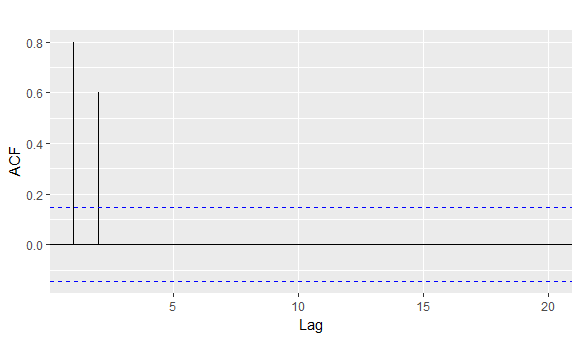
\includegraphics[width=.8\linewidth]{Images/Conceptos/ma_teorico.png}
  \caption{FAC de un proceso de medias móviles}
  \label{fig:sfig2}
\end{subfigure}
\caption{Correlogramas teóricos}
\label{comp_acf_pacf}
\end{figure}

\subsubsection{Estimación de los parámetros}
Una vez transformada la serie y seleccionado el modelo ARIMA a ajustar, es necesario estimar los parámetros. Existen multitud de métodos numéricos aplicados al cálculo de estos parámetros aunque quizás los más utilizados sean el método de máxima verosimilitud y el de mínimos cuadrados no lineales.

En ocasiones debido a problemas de no linealidad la maximización de la función de verosimilitud se realiza a través de métodos numéricos, es por esto por lo que el valor inicial de los parámetros es clave para garantizar una buena convergencia hacia el máximo. Existen varios métodos orientados al cálculo de estos valores (método de Yule-Walker, algoritmo de Burg, algoritmo de Hannan-Rissanen, etc…).

La potencia computacional necesaria para la estimación es tal que se resulta enormemente complicado realizar el cálculo manualmente. Generalmente no resulta necesario preocuparse por la estimación de los parámetros ya que se suele llevar a cabo automáticamente por rutinas ya implementadas en software estadístico especializado.

\subsubsection{Validación del modelo}
Una vez hemos elegido el modelo a ajustar y estimados sus parámetros debemmos comprobar si efectivamente se está realizando un buen ajuste, es decir, si nuestro modelo es válido.

Si el modelo ajustado explica correctamente nuestros datos no debemos esperarnos ningún tipo de patrón en los residuos, es decir, se deben comportar como ruido blanco. Una forma de comprobar esto es mediante la FAC y FACP de los residuos. Si esperamos que los residuos sean ruido no deberíamos observar correlaciones entre ellos, lo que significa que ninguna autocorrelación debería ser significativamente distinta de cero. Para comprobar esto definimos unas bandas de confianza al 95$\%$ para los correlogramas:
\begin{equation}
    \left[-\frac{1.96}{\sqrt{T}}, \frac{1.96}{\sqrt{T}}\right]
\end{equation}

\noindent siendo $T$ el número de valores de nuestra serie temporal.

Otra forma de estudiar los residuos es mediante la aplicación de test de contraste de hipótesis, los dos más usados son el de Box-Pierce y una variante de este conocida como Ljung-Box. Con estos estadísticos somos capaces de contrastar si las correlaciones entre los residuos son iguales a cero o no. Aunque ambos estadísticos funcionan bien en muestras grandes parece que el de Ljung-Box se comporta mejor en muestras pequeñas, es por esto lo que se ha extendido la utilización de este último:
\begin{equation}
   LB = T(T + 2) \sum_{k = 1}^{m} \frac{\hat{\rho}^2_{k}}{T-k}
\end{equation}

\noindent donde $\hat{\rho}_{k}$ es el coeficiente de autocorrelación de los residuos estimados hasta el retardo $k$ y $m$ el número de retardos sobre los que estamos trabajando. Este estadístico se distribuye bajo una Chi-Cuadrado con $m – p – q$ grados de libertad.

Además de los residuos conviene también tener en cuenta otros aspectos del modelo como la significatividad de los coeficientes o el poder predictivo. Al fin y al cabo es el investigador el que considera si el modelo es el correcto para sus datos.
	
Si el modelo no es válido se selecciona otro, se estiman los nuevos coeficientes y se vuelve a validar. El proceso se repite hasta que se encuentre un modelo que satisfaga las necesidades del investigador.

\subsubsection{Predicciones}
Una vez seleccionado y validado el modelo debemos predecir. Supongamos que hemos ajustado un ARMA($p, q$) a nuestra serie y queremos predecir $Y_{t + h}$, para ello debemos calcular:
\begin{equation}
    \widehat{Y}_{t + h} = a_{t + h} + \sum_{i=1}^{p} \widehat{\phi}_{i} \widehat{Y}_{t+h-i} + \sum_{i=1}^{q} (-\widehat{\theta}_{i}) a_{t+h-i}
\end{equation}

\noindent donde $a_{t + h} = 0$, $\widehat{Y}_{t+h-i}$ son las predicciones realizadas en tiempos anteriores y $a_{t+h-i}$ los residuales de esas predicciones. Se puede apreciar como para calcular la parte autorregresiva y medias móviles de la serie en el tiempo $t + h$ se ha necesitado realizar las predicciones para los tiempos $t+1,...,t+h-1$.

Es posible calcular los intervalos de confianza de estas predicciones, pero para ello tenemos que asegurarnos de que los residuos sean ruido, en caso contrario puede que los intervalos sean erróneos. Estos intervalos se amplían a medida que nos alejamos en las predicciones, llegando a converger en horizontes lejanos de la serie.
